%!TEX root = ../../Main.tex
\graphicspath{{Chapters/Diskussion/}}
%-------------------------------------------------------------------------------


\section{Systemarkitektur}


Vores systemarkitektur fungerer som den overordnede ramme for hvordan vi senere har implementeret vores system. Dette afsnit vil give et overblik over vores systems arkitektur, for at give et overskueligt overblik over systemet. Det er her at den beskrevne funktionalitet deles ud i mindre moduler. 

\subsection{Blokidentifikation}
På figur \autoref{fig:ColorSortingSystem_BDD}  ses det overordnede BDD, som beskriver de enkelte moduler som systemet indeholder. Hver blok beskriver en funktionalitet, som systemet håndterer. I det følgende vil de enkelte moduler og funktionalitet kort beskrives.

\begin{figure}[H]
	\centering
	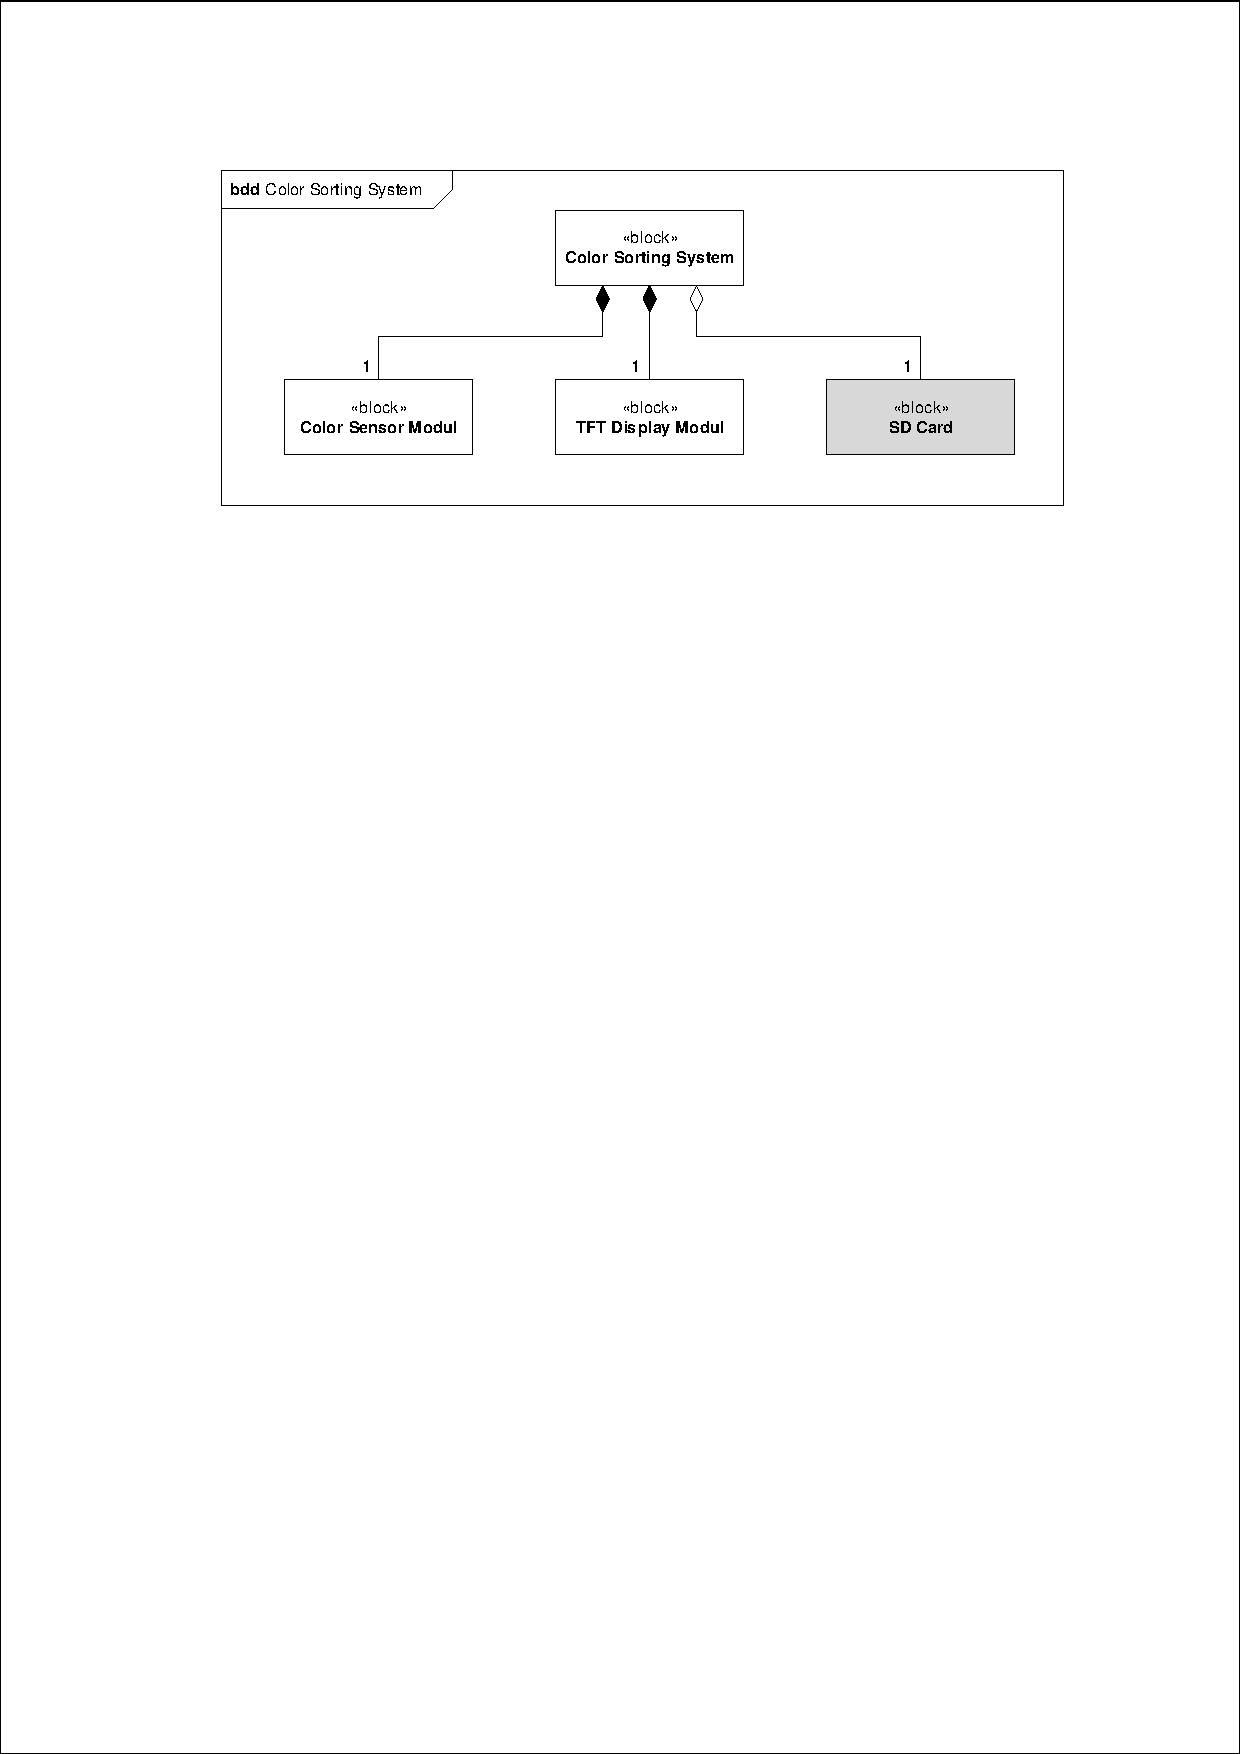
\includegraphics[width = 400pt]{Img/ColorSortingSystem_BDD.png}
	\caption{Color Sorting System BDD}
	\label{fig:ColorSortingSystem_BDD}
\end{figure}

\textbf{TFT Display Module:} \\
Har til opgave at modtage data fra Color Sensor Module og vise brugeren på baggrund af det modtaget data, antallet af hver enkelt farve målt, samt det totale antal farver. Dette modul skulle også havde haft ansvaret for at sende data til SD-kortet, hvis den del var blevet implementeret. 
\\\textbf{Color Sensor Module:} \\
Har til opgave at måle farven placeret under Color Sensoren, samt sende informationen videre til TFT Display Module.
\\\textbf{SD-Kort:}\\
Et SD kort som var tiltænkt at kunne opbevare data som efter systemet slukkes. Dette blev dog taget ud af system. Hvilket visualiseres ved den grå farve i BDD’et.  

\subsection{Blokinteraktion}

På \autoref{fig:ColorSortingSystem_IBD} nedenfor ses det overordnede IBD for systemet. IBD’et viser de forskellige hardwareblokke i systemet og deres interaktion mellem hinanden. Interaktionen mellem blokkene bliver beskrevet mere detaljeret under dokumentationen for de enkelte blokke. I forhold til det overordnede BDD på \autoref{fig:ColorSortingSystem_BDD} har vi valgt at vise hvilke hardware blokke de enkelte moduler består af, for at give et indblik i interaktionen internt i modulerne. 

\begin{figure}[H]
	\centering
	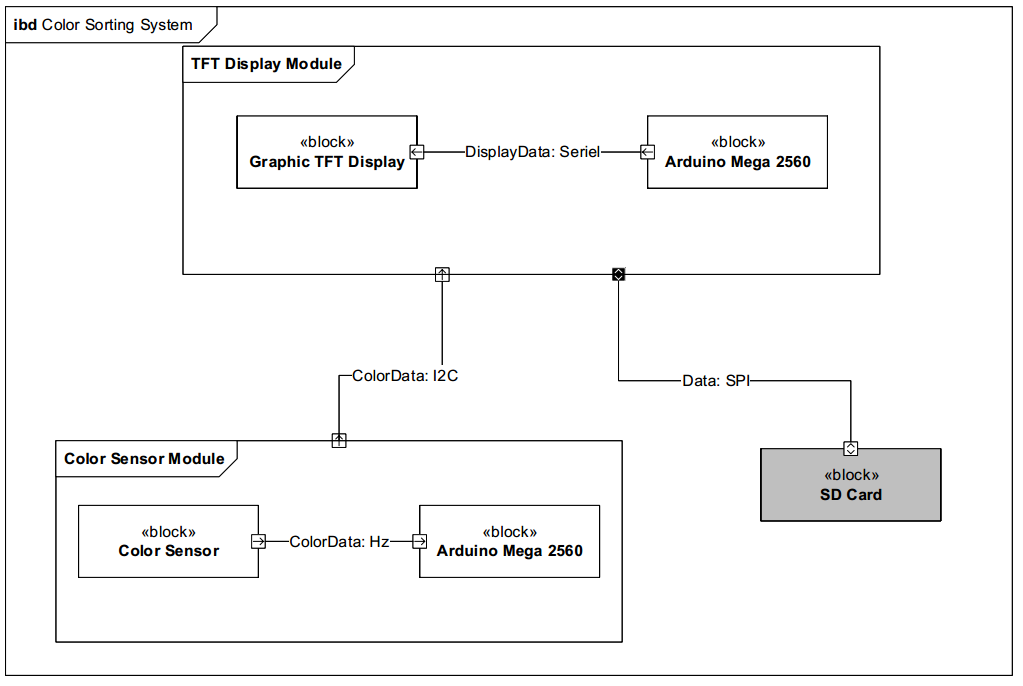
\includegraphics[width = 500pt]{Img/ColorSortingSystem_IBD.png}
	\caption{Color Sorting System IBD}
	\label{fig:ColorSortingSystem_IBD}
\end{figure}